%\documentclass[xcolor={dvipsnames}]{beamer}

\documentclass[xcolor={dvipsnames}, notes]{beamer}

\usetheme{Warsaw}

\usepackage{inputenc}
\usepackage{amsmath}
\usepackage{theorem}
\usepackage{graphicx}
%\usepackage{geometry}
\usepackage{tasks}
\ifodd\textwidth
  \addtolength{\textwidth}{1sp}
\fi


\newcommand{\po}{\textcolor{BlueViolet}{po}}
\newcommand{\rf}{\textcolor{Green}{rf}}
\newcommand{\co}{\textcolor{BurntOrange}{co}}
\newcommand{\mo}{\textcolor{Red}{mo}}
\newcommand{\hb}{\textcolor{NavyBlue}{hb}}
\newcommand{\fr}{\textcolor{RubineRed}{fr}}
\newcommand{\xhb}{\textcolor{NavyBlue}{xhb}}
\newcommand{\rfe}{\textcolor{Green}{rfe}}
\newcommand{\rfi}{\textcolor{Green}{rfi}}
\newcommand{\sw}{\textcolor{BurntOrange}{sw}}
\newcommand{\jhb}{\textcolor{NavyBlue}{jhb}}
\newcommand{\jmo}{\textcolor{Red}{jmo}}
\newcommand{\eco}{\textcolor{WildStrawberry}{eco}}


\title{Axiomatic Memory Model Specifications}

\author{Akshay Gopalakrishnan (self Reference material)}

\begin{document}

    \begin{frame}
        \maketitle
    \end{frame}
    %First section should elicit the preliminary definitions needed to define these models.
    %Specific models may have additional definitions and we can contain them in their respective sections. 

    \begin{frame}{Preliminary Definitions}
        
        Language syntax: 
        \begin{align*}
            & E ::= \ r \ | \ v \ | \ X \ | \ E+E \ | \ E*E \ | \ E\leq E \ | \ ... \\
            & C ::= \ skip \ | \ C;C \ | \ r=E \ | \ r=X \ | \ X=E \ | \ r=RMW(X,E,E) \ | \ r=RMW(X,E) \\
            & | \ br \ label \ | \ br \ label \ label \ |... \\
            & P ::= \ X=v;...;X=v;\{C|...|C\}
        \end{align*}

        In the above syntax:
        \begin{itemize}
            \item $X \in Locs$ - Where Locs is a map of the shared memory on which programs will operate.
            \item $r \in Reg$ - Where Reg is the set of registers per thread.
            \item $v \in Val$ - Where Val is the set of literals. 
        \end{itemize}

    \end{frame}

    \begin{frame}{Preliminary Definitions cnt'd}
        
        Given a binary relation $R$, here are the useful variants for our purpose:
        \begin{itemize}
            \item $R^{-1}$ - Inverse relation $\langle a, b\rangle \in R \ \Rightarrow \ \langle b, a\rangle \in R^{-1}$.
            \item $R^{?}$ - Reflexive relation $\langle a, a\rangle \in R$. 
            \item $R^{+}$ - Transitive relation $\langle a, b\rangle \in R \ \wedge \ \langle b, c\rangle \in R \ \Rightarrow \ \langle a, c\rangle \in R$. 
            \item $R^{*}$ - Reflexive Transitive relation $R^{+} U R^{?}$.
            \item $R1;R2$ - Sequential composition $\langle a, b\rangle \in R1 \ \wedge \ \langle b, c\rangle \in R2 \ \Rightarrow \ \langle a, c\rangle \in R1;R2$
            \item $[R]$ - Identity relation $\langle a, b\rangle \in R \ \Rightarrow \ a=b$.
            \item $dom(R)$ - Domain of $R$.
            \item $codom(R)$ - Range of $R$.
        \end{itemize}
    
    \end{frame}
    
    \begin{frame}{Preliminary Definitions cnt'd}
        
        Event is:
        \begin{itemize}
            \item Of the form $\langle id, tid, lab \rangle$.
            \item $id$ - Unique identifier distinguishing event in the whole program.
            \item $tid$ - Thread identifier distinguishing event in its own thread.
            \item $lab = \langle op, loc, rval, wval \rangle$ - Event label specifying the operation and the memory/fence involved.  
                \begin{itemize}
                    \item $op ::= \ Ld \ | \ St \ | \ U \ | \ F.$ - Load, Store, Update or Fence.
                    \item $loc$ - Memory location on which the operation is.
                    \item $rval$ - Read value of the operation.
                    \item $wval$ - Write value of the operation. 
                \end{itemize}
        \end{itemize}

    \end{frame}
    
    \begin{frame}{Preliminary Definitions cnt'd}
        
        Axiomatic events:
        \begin{itemize}
            \item Read event $\Re = Ld \cup U$.
            \item Write event $W = St \cup U$. 
            \item Fence - Can be of various types depending on the architecture / language's memory model.
        \end{itemize}

        Binary relations:
        \begin{itemize}
            \item {\po} - Program order per thread.
            \item {\rf} - Between a read and the write from which its read value comes.
            \item {\co} - Order between writes/updates to same location.
            \item {\mo} - Order between memory writes/updates.
        \end{itemize}

    \end{frame}
    
    \begin{frame}{Sequential Consistency (SC)}
        
        Additional binary relations:
        \begin{itemize}
            \item {\hb} - Happens before $ \hb = (\po \cup \rf)^{+} $
            \item {\fr} - Reads before (from reads) $ \fr = (\rf^{-1};\mo_{|loc}) $ 
        \end{itemize}

        SC is defined using the following irreflexivity relations that must hold for any program execution:
        \begin{tasks}(2)
            \task {\mo} irreflexive and total.
            \task {\hb} irreflexive.
            \task {\mo;\hb} irreflexive.
            \task {\fr;\hb} irreflexive.
            \task {\fr;\mo} irreflexive.
            \task {\fr;\mo;\hb} irreflexive.
        \end{tasks}

    \end{frame}

    \note{
        The above model is equivalent to the acyclic model of SC, which is 
        $(\po \cup \rf \cup \mo \cup \fr)$ acyclic.
        Because $(\po \cup \rf)$ is {\hb}, the above definition becomes 
        $(\hb \cup \mo \cup \fr)$ acyclic.
        This acyclic condition can be divided into the above 6 irreflexivity conditions (just pick them in combination, and they must be irreflexive).
        A simple permutation of sets and property of acyclic binary unions.
        The next slide does in fact show graphs of these cases for better intuition.          
    }

    \begin{frame}{Figures to explain above axioms of irreflexivity}
        
        \begin{figure}
            \makebox[\textwidth][c]{
                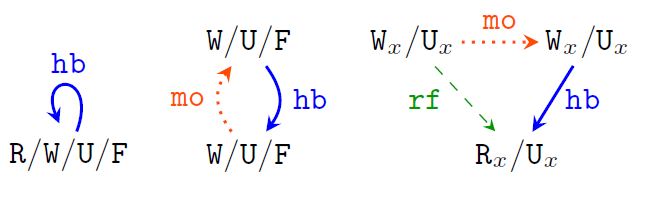
\includegraphics[scale=0.5]{SC-Def1.PNG}
            }
        \end{figure}

        \begin{figure}
            \makebox[\textwidth][c]{
                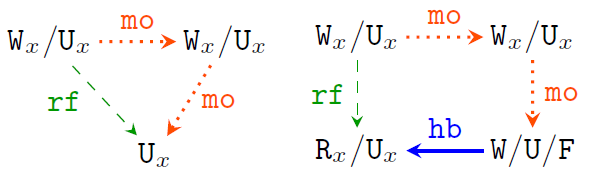
\includegraphics[scale=0.5]{SC-Def2.PNG}
            }
        \end{figure}

    \end{frame}

    
    \begin{frame}{x86 Total Store Order (TSO)}
        
        Additional binary relations:
        \begin{itemize}
            \item {\xhb} - Happens before $ \xhb = (\po \cup \rf)^{+} $
            \item {\fr} - Reads before (from reads) $ \fr = (\rf^{-1};\mo_{|loc}) $ 
            \item {\rfe} - Reads from external $\rf \text{ \textbackslash} \ \po$
        \end{itemize}

        x86 TSO is defined using the following irreflexivity relations that must hold for any program execution:
        \begin{tasks}(2)
            \task {\xhb} irreflexive.
            \task {\mo;\xhb} irreflexive.
            \task {\fr;\xhb} irreflexive.
            \task {\fr;\mo} irreflexive.
            \task {\fr;\mo;\rfe;\po} irreflexive.
            \task {\fr;\mo;$[U \cup F]$;\po} irreflexive.
        \end{tasks}

    \end{frame}
    
    \note{
        The last two rules show the difference betweeen TSO and SC. 
        Basically, they ONLY restrict read values from main memory to be that of the last written value. 
        But, cases where a read takes value from its own thread's write buffer is perfectly fine.
    }

    \begin{frame}{Figures to explain the last two axioms of irreflexivity.}
            
        \begin{figure}
            \makebox[\textwidth][c]{
                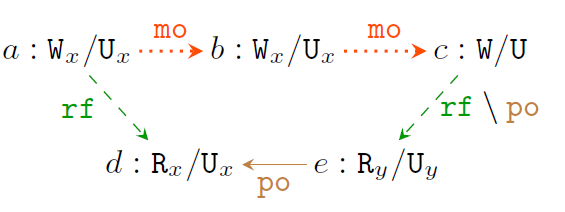
\includegraphics[scale=0.5]{TSO-Def1.PNG}
            }
        \end{figure}

        \begin{figure}
            \makebox[\textwidth][c]{
                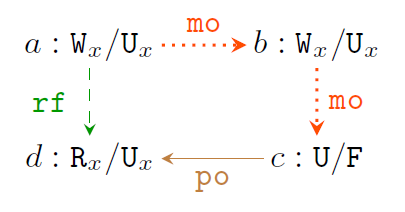
\includegraphics[scale=0.5]{TSO-Def2.PNG}
            }
        \end{figure}

    \end{frame}
    
    %Mapping from SC --> x86-TSO
    \begin{frame}{Mapping from SC to TSO}

        \begin{itemize}
            \item SC Load --- TSO Load $LD \mapsto LDR$.
            \item SC Store ---- MFENCE;TSO Store $ST \mapsto MFENCE;STR$.
        \end{itemize}

        %\begin{theorem}
            The above mapping from SC ---> TSO is correct.
        %\end{theorem}
        %We will consider RMW later. 
        
    \end{frame}

    \begin{frame}{Mapping from SC to TSO : Proof Statement}

        Consider $P_{SC}$ and $P_{TSO}$ to be programs corresponding to each memory model such that the above mapping is applied $P_{SC} \mapsto P_{TSO}$.
        Let us consider $X_{SC}$ and $X_{TSO}$ to be the respective consistent executions under the memory models.
        Then, the following holds true
        \begin{align*}
            P_{SC} \mapsto P_{TSO} \ \implies \ \forall X_{TSO} \ \exists X_{SC} \ \textit{s.t.} \ B(X_{SC}) = B(X_{TSO}). 
        \end{align*}
        where $B$ is a function that maps an execution to its corresponding observable behavior (reads-from relations).
        
    \end{frame}

    \begin{frame}{Proof idea}
        
        We do it using proof by contradiction.

        We take one execution $X_{TSO}$ which is consistent.
        If the above proof statement is to be false, then the same execution must have been illegal under $SC$, $X_{SC}$ is not consistent.
        Inconsistent execution would mean that one of the irreflexivity axioms of $SC$ fails to hold, while all of those of $TSO$ holds.

        We prove that this is not the case, by showing that if it is inconsistent in $SC$, it is inconsistent in $TSO$ as per the mapping.
        
    \end{frame}

    \begin{frame}{Proof cnt'd}

        Firstly, note that the following relations of $SC$ are contained in $TSO$
        \begin{tasks}(2)
            \task \po
            \task \rf
            \task \mo
            \task \hb
            \task \fr
        \end{tasks}

        From the above, and by the property that if a sequential composition is irreflexive and contains another composition, then the latter also is irreflexive.
        \begin{align*}
            R1 \subseteq R2 \ \wedge \ R2 \ \text{irreflexive} \ \implies \ R1 \ \text{irreflexive}.
        \end{align*}
        
        Thus the following axioms hold for $SC$ too:
        \begin{tasks}(2)
            \task {\hb} irreflexive.
            \task {\mo;\hb} irreflexive.
            \task {\fr;\hb} irreflexive.
            \task {\fr;\mo} irreflexive.
        \end{tasks}

        Note: {\mo} remains a strict total order the same way.

    \end{frame}

    \begin{frame}{Proof cnt'd}
        
        Now what remains is the last axiom of $SC$ - ${\fr;\mo;\hb}$
        Assume that $X_{SC}$ does fail due to this axiom.
        Thus, we have ${\fr;\mo;\hb}$ to be reflexive. 
        Then, the resulting composition due ot mapping to $TSO$, must also be reflexive 
        \begin{align*}
            &{\fr;\mo;\hb} \\
            &{\fr;\mo;[ST];\hb} \\
            &{\fr;\mo;[F;STR];\xhb}  
        \end{align*}

        $\fr;\mo;[F;STR];\xhb$ has following 3 variants due to {\xhb}.
        \begin{tasks}(2)
            \task {\fr;\mo;[F];\po}.
            \task {\fr;\mo;\rfe;\po}.
            \task {\fr;\mo;\rfi;\po}.
            \task beee
        \end{tasks}
        
    \end{frame}

    \begin{frame}{Proof cnt'd}
        
        \begin{enumerate}
            \item {\fr;\mo;[F];\po} is irreflexive as $X_{TSO}$ is consistent.
            \item {\fr;\mo;\rfe;\po} is irreflexive as $X_{TSO}$ is consistent.
            \item {\fr;\mo;\rfi;\po} is irreflexive as {\xhb} is irreflexive. 
        \end{enumerate}

        %The last case boils down to \rfi;\po, but this is equivalent to just \po, which then becomes case 1
        Both possibilities $\fr;\mo;\rfe;\po$ and $\fr;\mo;[F];\po$ are axioms of $TSO$ which are irreflexive.
        The third case is a subset of the first. 
        Thus, by contradiction, we can infer $\fr;\mo;\hb$ is irreflexive.
        Hence, proved.

    \end{frame}

    %Fence optimizations (elimination optimization)
    \begin{frame}{Fence elimination in x86-TSO}

        Categorize fences as eliminable and non-eliminable.
        Often it is easier to specify fences which are non-eliminable.
        Doing so will also give us the condition (direct negation) on which Fence Optimization can be done.

        
        \centering \textit{An \emph{MFENCE} in an x86 program is non-eliminable if it is the only fence in the program path from a store to a load in the same thread.} 
        
        %This allows reordering of store-load pairs each of which work on disjoint memory.
        %So if the user wants the specific store load pair to not change, one needs to add an MFENCE. 
        %In all other cases, the MFENCE is not particularly needed, so can be safely eliminated.
        %The intuition behind this is unclear, but must come accross while proving this optimization as sound under TSO.
    \end{frame}

    \note{
        \begin{enumerate}
            \item Store-Store need to be ordered per thread under TSO (as the write buffer is also ordered)
            \item Load-Load need to be ordered as the first Load would influence the second load value (axiomatically one can think of this as happens-before).
            \item Load-Store also needs to be ordered as the load would imply an ordering between the subsequent store and stores from other threads (if load is from Main Memory, this would make visible the current write value which is going to be overwritten by the subsequent write).
            \item Store-Load however, does not have any reason to be ordered. A load from main memory would imply that the previous store is not relevant and could be in write buffer or could be updated in main memory. This choice is independant of when the following load is done. 
        \end{enumerate}
    }

    \begin{frame}{Proof idea}
        
        We have the fence elimination transformation from $P_{src}$ to $P_{trgt}$.
        Taking theorem of correct compiler mapping, we have:
        \begin{align*}
            P_{src} \ \mapsto \ P_{trgt} \ \implies \ \forall X_{trgt} \in P_{trgt}. \exists X_{src} \in P_{src}. B(X_{src}) = B(X_{trgt}).
        \end{align*}

        This means, considering a target execution which is consistent, if we perform a de-transformation to get the source execution, which must have the same behavior.
        If not, then it would mean that the source execution is inconsistent. %little doubtful about this implication
        Which means one of the irreflexivity constraints fail to hold. 
        This we can prove by contradiction that it does indeed hold.
        
        %Since this works directly at the candidate execution level, this seems a little off. 
        %Doing a transformation would certainly be valid only if the target program's behaviors are contained in that of the source.
        %But the definition of behavior, kept only as the read values, can be justified in other ways too. 
        %If we have multiple writes in one program and we perform a transformation that would disallow one reads-from relation, it could be that the target program justifies it using another set of reads-from relation, thus keeping the read value same. 
        %This would be more problematic in the compiler mapping case, as we clearly have different memory models.

        %Checking the proof for reordering or elimination would tell us something.

    \end{frame}

    \note{
        To prove that the transformation is safe, note that the transformed program's behaviors should at least be contained (if not equal) in that of the original ($P_{trgt} \subseteq P_{src}$). 
        If we consider the source code and perform a transformation $P_{src} \mapsto P_{trgt}$, then we have a similar property as that of compiler mapping $\forall X_{trgt}.\exists X_{src}.O(X_{trgt}) = O(X_{src})$.
        We can prove this straightforward by contradiction, as if there does not exist a source execution, it would only mean that it is illegal, as we know behaviors must be contained. 
        Which means one of the irreflexivity conditions fail to hold, which we can verify similar to the compiler mapping proof.
        This is a very intelligent way to proving transformations, one that I did not know back then.
        This also solves my doubt of why a de-transformation is considered while proving program transformation.
        Also, this method seems to be independent of the transformation done, which greatly helps in our case. 
    }



    %Proof details
    \begin{frame}{Proof}
        Assume that indeed for some $X_{trgt}$, $X_{src}$ does not exist. 
        This would mean the resulting $X_{src}$ is inconsistent. 

        Case 1: 
        \begin{align*}
            & \xhb \ \textit{irreflexive}.\\
            & \xhb;[F];\xhb. \\ 
            & \xhb;[E];\po;[F];\po;[E];\xhb. \\ 
            & \xhb;[E];\po;[E];\xhb. \\
            & \xhb. %Of trgt should also be reflexive.
        \end{align*}

        Case 2:
        \begin{align*}
            & \fr;\xhb.\\
            & \fr;[W];\po\xhb;[F];\xhb. \\ 
            & \fr;[W];\xhb. \\ 
            & \fr;\xhb. \\ %Of trgt should also be reflexive.
        \end{align*}

    \end{frame}

    \note{For Case 1, note that if a cycle exists, $[F]$ must be a part of it. 
    Also note that, this $[F]$ and {\xhb} relations with it are formed through direct program order relations, which must, by transitive property also be part of the cycle.
    However, this also means, the set of events without $[F]$ also should form a cycle, which is a contradiction as $X_{trgt}$ is consistent.
    For Case 2, note that again, it implies a cycle must exist without $[F]$ being involved. 
    Thus by contradiction Case 1 and Case 2 are eliminated. }

    \begin{frame}{Proof cnt'd}

        Case 3:
        \begin{align*}
            \mo;\xhb;
        \end{align*}

        Two sub-cases:
        \begin{align*}
            & \mo;[F];\xhb. \\ %W-mo-F-xhb-W.
            & \mo;[F];\po;[E];\xhb. \\ %Cannot have direct relation with relations other than ones immediately following/Preceding in po.
            & \mo;[W];\xhb. \\ %Should also be cyclic then for X_{trgt}
            \\
            & [F];\mo;\xhb;[F].\\ %F-mo-E-xhb-F --> F-mo-E
            & [F];\mo;\xhb;[R];\po;[F].\\ %As direct relations do not come to [F] apart from those po after/preceding.
            & [F]\xhb;[W];\mo;\xhb;[R];\po;[F].\\ %As mo implied relations cannot exist unless an xhb edge is contained.
            & [W];\mo;\xhb;[W]. %Should also be a cycle for X_{trgt}.
        \end{align*}
    
    \end{frame}

    \note{For Case 3, note that apart from the naive transitive relations that imply to $X_{trgt}$ to have cycles, we can also have $[F]$ such that it links {\mo} and {\xhb}, thus introducing a cycle. 
    In the first case, $[F]$ is the codomain of {\mo} and domain of {\xhb}. However, note that {\xhb} relations with $[F]$ cannot be direct, and must come from some event {\po} ordered after it. Thus, by transitivity, requiring that there also exists a cycle without the fence. 
    The same reasoning is used for the second case, with the added observation that {\mo} edges cannot exist with $[F]$ unless there also exists {\xhb} relation. This might sound a bit difficult to grasp, but on drawing example graphs, the intuition will be more clear. The crux is that there is no \textit{direct} edge of {\mo} or {\xhb} with $[F]$ unless its derived from {\po}.}

    \begin{frame}{Proof cnt'd}

        Case 4:
        \begin{align*}
            &\fr;\mo.\\
            &\fr;[W];\mo;[F];\mo.\\
            &\fr;[W];\mo.\\
            &\fr;\mo. %Of trgt should be reflexive.
        \end{align*}

        Case 5: 
        \begin{align*}
            &\fr;\mo;\rfe;\po.\\
            &\fr;\mo;\rfe;\po. %Of trgt should be reflexive. \mo , \po is irreflexive and fence cannot be placed between \fr;\mo and \rfe;\po 
        \end{align*}

    \end{frame}

    \note{Case 4 and 5 have no case (apart from transitive relations) for having cycles with $[F]$. Thus, both cases are eliminated.}

    \begin{frame}{Proof cnt'd}

        Case 6:
        This case is tricky.
        \begin{align*}
            &\fr;\mo;[F];\po.\\
            &\fr;\mo;[W];\mo;[W];\xhb;[F];\po.\\ 
            &\fr;\mo;[W];\mo;([W];\rfe;\po \ \cup \ \po);[F];\po.
        \end{align*}

        Two sub-cases to this.
        \begin{align*}
            &\fr;\mo;[W];\mo;[W];\rfe;(\po;[F];\po).\\
            &\fr;\mo[W];\mo;[W];\rfe;\po.\\
            &\fr;\mo;\rfe;\po.\\ %Should be reflexive for X_{trgt} too.
            \\
            &\fr;\mo;[W];\mo;[W];\po;[F];\po.\\
            &[R];\fr;\mo;[W];\mo;[W];\po;[F];\po;[R].\\
            %Now if [F] is the only fence there, then that one is non-eliminable, thus, we have.
            &\fr;\mo;[F];po.\\ %For X_{trgt} to also be reflexive. By contradiction, X_{src} is irreflexive.
            %If [F] is not the only fence there, then also the above holds after eliminating the fence. 
            &\fr;\mo;[F];\po;[F];\po.\\
            &\fr;\mo;[F];\po.\\ % For X_{trgt} to also be reflexive. By contradiction, X_{src} is irreflexive.
        \end{align*}
            
    \end{frame}

    \note{Firstly, note that there cannot be any direct relation W-mo-F unless W-po-F.
    The reason is because of the definition of happens before between two threads, which only is formed between reads and writes.
    And because of the reads-from-external, a memory order is implied between writes, but not fences.
    So a case like $w-f-r||w'$, where $w'-rf-r$, it implies $w-w'$, but nothing with the fence.
    If, however, we have like w-mo-w'-xhb-f, then we can infer that w-mo-f.
    The two sub-cases are a result of the above observation. 
    The first requires that $X_{trgt}$ is also reflexive, thus eliminating this case by contradiction. 
    The latter, is the tricky case.
    Firstly, if $[F]$ is the only fence, it counts as non-eliminable.
    If it isn't then, by transitivity, we again have the same composition(final expression) to also be a cycle in $X_{trgt}$. 
    Thus by contradiction, this case also is eliminated.
    }

    %JavaScript Memory model
    \begin{frame}{JavaScript Memory Model}
        
        Additional type for each memory access - Unordered($uo$)|Initialize($init$)|SequentiallyConsistent($sc$)
        \begin{itemize}
            \item $W \ ::= \ uo|init|sc $.
            \item $R \ ::= \ uo|sc $.
            \item $RMW \ ::= \ sc$
        \end{itemize}

        Memory location(s) have three forms - Disjoint($dj$)|Overlap($op$)|Equal($eq$)
        Wherever relevant, in a binary relation we will use the above three forms.
        
        Additional Binary Relations:
        \begin{itemize}
            \item {\sw} - Synchronize-with $po \ \cup \ ([W_{sc}];\rf;[R_{sc}])_{eq}$
            \item {\jhb} - Happens before $\sw \ \cup \ \{\langle a,b \rangle | a = W[init] \ \wedge \ b=W|R|RMW \ \wedge \ ([a];\xhb;[b])_{op} \}$
            \item {\jmo} - Memory order (total order of all events in execution) 
        \end{itemize}

        
    \end{frame}

    %Irreflexivity constraints
    \begin{frame}{JavaScript Memory Model: Axioms}
        
        \begin{tasks}(2)
            \task {\jhb} irreflexive.
            \task {\jhb;\jmo} irreflexive.
            \task {\jhb;\rf} irreflexive.
            \task {$(\fr;\xhb)_{op}$} irreflexive.
        \end{tasks}

        \begin{enumerate}
            \item {$(([R_{sc}];\fr;[W_{sc}])_{eq};\mo;[W'_{sc}];\mo)_{eq}$} irreflexive.
            \item {$([W_{sc}];\jhb;[R];\fr;[W'_{sc}])_{eq};\jhb;[R];\rf^{-1}$} irreflexive. %Since rf-1 is not functional in nature, we would need some additional conditions for mixed size. 
            \item {$[W];\jhb;([R_{sc}];\fr;[W'_{sc}])_{eq};\jhb;[R_{sc}];\rf^{-1}$} irreflexive.
        \end{enumerate}
        %W,W' is sc and R can be any. W-hb-R and W'-hb-R and W-mo-W'-mo-R and W-rf-R is not allowed and W,W' eq range
        % W-hb-R-fr-W'-hb-R-rf^{-1}
        %W',R is sc and W can be any. W-hb-W' and W-hb-R and W-mo-W'-mo-R and W-rf-R is not allowed and W',R eq range
    \end{frame}

    %C11 memory model
    \begin{frame}{C11/C++ Memory Consistency Model}
        Additional binary relations:
    \end{frame}

    %Irreflexivity constraints


\end{document}